\documentclass[class=report, crop=false, a4paper, 12pt]{standalone}

%Packages import
\usepackage{../pkgs}


\begin{document}
\newpage
% A face recognition system works in either or both of two modalities: face verification (or authentication) or face identification (or recognition). The difference between them lies in the final stage of the workflow, identification involves a one-to-one pairing, while identification is a one-to-many match.

\section{Face Recognition}
Face Recognition (FR) is a thoroughly debated and extensively researched task in the Computer Vision community for more than two decades \autocite{ranjanDeepLearningUnderstanding2018}, popularized in the early 1990s with the introduction of the Eigenfaces \autocite{turkEigenfacesRecognition1991} or Fisherfaces \autocite{p.n.belhumeurEigenfacesVsFisherfaces1997} approaches. These methods projected faces in a low-dimensional subspace assuming certain distributions, but lacked the ability to handle uncontrolled facial changes that broke said assumptions, henceforth, bringing about face recognition approaches through local-features \autocite{chengjunliuGaborFeatureBased2002, ahonenFaceDescriptionLocal2006} that, even though, presented considerable results, weren't distinctive or compact. Beginning in 2010, methods based on learnable filters arose \autocite{z.caoFaceRecognitionLearningbased2010,leiLearningDiscriminantFace2014}, but unfortunately revealed limitations when nonlinear variations were at stake.

\par Earlier methods for FR worked appropriately when the data was handpicked or generated on a constrained environment, however, they didn't scale adequately in the real world were there are large fluctuations in, particularly, pose, age, illumination, background scenario, the presence of facial occlusion \autocite{ranjanDeepLearningUnderstanding2018} and many unimaginable more. These shortcomings can be dealt with by using Deep Learning, a framework of techniques that solves the nonlinear inseparable classes problem \red{ref.}, more specifically a structure called Convolutional Neural Network (CNN) \autocite{wangDeepFaceRecognition2021}. 

\par CNNs are an Artificial Neural Network (ANN) that exhibit a better performance on image or video-based tasks compared to other methods \autocite{lecunGradientBasedLearningApplied1998}. They were greatly hailed in 2012, after the AlexNet \autocite{krizhevskyImageNetClassificationDeep2012} victory, by a great margin, in the ImageNet Large Scale Visual Recognition Challenge (ILSVRC). Just two years later, DeepFace \autocite{taigmanDeepFaceClosingGap2014} revolutionized the benchmarks scores by achieving state-of-the-art results that approached human performance, reinforcing even further the importance of Deep Learning and shifting the research path to be taken \autocite{wangDeepFaceRecognition2021}.

\par Given what has been stated so far and the proven robustness, performance, and overall results in computer vision \red{ref. won competitions}, the methods discussed in this dissertation will therefore deal exclusively with Deep Learning approaches. For more information on other methods, please refer to \autocite{learned-millerLabeledFacesWild2016}.
% The exponential growth in the Artificial Intelligence domain, its corresponding subfields and technologies involved, spanned a plethora of terms that can be easily confused, mistook or mixed. For a better understanding of this dissertation, before discussing methods and implementations, it's important to analyze the fundamentals.


% \vspace{0.7\baselineskip}
% \noindent\textbf{$\rightarrow$ Computer Vision} is the science of trying to mimic with a computer what the humans do when looking at a scene, that is, extracting information from images through a series of computational techniques. \autocite{szeliskiComputerVisionAlgorithms2022}

% \vspace{0.7\baselineskip}
% \noindent\textbf{$\rightarrow$ Image querying}, is the process of finding information in a database of images that corresponds to the user query\footnote{Query, in computer science, is the request for information in a database.}, in this case, an image query\autocite{bartoliniImageQuerying2009}.  

\section{A Face Recognition System}

\begin{figure}[!h]
    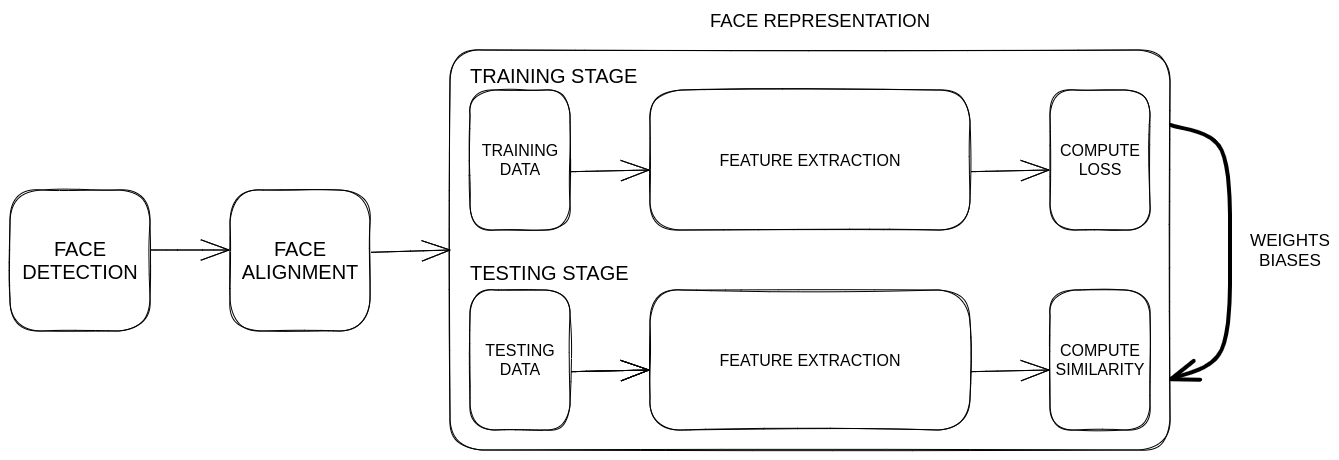
\includegraphics[scale=0.30]{fr_pipeline.png}
    \caption[Pipeline]{A typical face recognition pipeline, guided by the approach in \autocite{wangDeepFaceRecognition2021}.}
    \label{fig:fr pipeline}
\end{figure}

\par According to Ranjan \textit{et al.} \autocite{ranjanDeepLearningUnderstanding2018}, the goal of a FR system is to find, process and learn from a face, gathering as much information as possible, and as a result, it is one of the most widely implemented biometric system solutions in light of its versatility when facing real world application \autocite{duElementsEndtoendDeep2022}, such as \red{military, public security and daily life}.

\par By and large, all end-to-end automatic face recognition systems follow a sequential and modular\footnote{Sequential because each stage relies on the output from the previous ones, and modular in the sense that each stage employs its own method and it can be modified to better adapt to specific tasks.} pipeline \reffig{fig:fr pipeline} composed of three pillar stages \autocite{wangDeepFaceRecognition2021}: face detection, face alignment and face representation. First an image or video feed is used as an input then, as the name suggests, the \textbf{face detection} module is responsible for finding a face. Next, the \textbf{face alignment} phase applies spatial transformations to the data in order to normalize the faces' pictures (or frames, in the case where a video is used) to a standardized view. Finally, the \textbf{face representation} stage, makes use of deep learning techniques to learn discriminative features that will allow the recognition.

\par All three stages have their individual importance and methods of implementation\footnote{For a deeper and extensive study, please refer to: \autocite{zafeiriouSurveyFaceDetection2015} in the case of classic face detection approaches and \autocite{minaeeGoingDeeperFace2021} for deep learning based methods; \autocite{wangFacialFeaturePoint2018} addresses traditional face alignment methods and is complemented with \autocite{duElementsEndtoendDeep2022} for more up-to-date techniques; and \autocite{learned-millerLabeledFacesWild2016} tackles classic face representation \red{(add the following if needed) while X supplements the deep learning ones.}}. \textbf{Face detection} is achievable through classical approaches \autocite{violaRapidObjectDetection2001, brubakerDesignCascadesBoosted2008} or deep methods, among them is \autocite{dengRetinaFaceSinglestageDense2019} and the widely applied \autocite{zhangJointFaceDetection2016a}. \textbf{Face alignment}, once again, can be accomplished through traditional measures \autocite{cootesViewbasedActiveAppearance2002, martinezLocalEvidenceAggregation2013} or more modern ones, namely \autocite{huangPropagationNetPropagatePoints2020} or the aforementioned \autocite{zhangJointFaceDetection2016a} which concurrently performs detection and alignment. To conclude, the \textbf{face representation} module is no exception, and can also be divided in two groups, regarding the methodology used. Some conventional systems were already mentioned, such as \autocite{p.n.belhumeurEigenfacesVsFisherfaces1997,turkEigenfacesRecognition1991}, and the deep learning ones are the object of discussion of this dissertation and will be reviewed along the following sections, therefore, the focus will be on describing, with particular interest, the face representation stage.

\subsection{Face Detection}
\par Face detection is the first step in any automatic facial recognition system. Given an input image to a face detector module, it is in charge of detecting every face in the picture and returning bounding-boxes coordinates, for each one, with a certain confidence score \autocite{duElementsEndtoendDeep2022,ranjanDeepLearningUnderstanding2018}.

\par Previously employed traditional face detectors \red{cite here} are incapable of detecting facial information when faced with challenges such as variants in image resolution, age, pose, illumination, race, occlusions or accessories (masks, glasses, makeup) \autocite{duElementsEndtoendDeep2022,ranjanDeepLearningUnderstanding2018}. The progress in deep learning and increasing GPU power led DCNNs to become a viable and reliable option that solves said problems in face detection. 

\par These techniques can be included in different categories. A more analytical perspective \autocite{duElementsEndtoendDeep2022} distributes the methods, depending upon their architecture or purpose of application, over seven categories: multi-stage, single-stage, anchor-based, anchor-free, multi-task learning, CPU real-time and, finally, problem-oriented. Additionally, being as the face detection problem can be seen as a specific task in a general object detection situation, it is no surprise that several works inherit from them and, therefore, some bases are referenced throughout the next list.

\vspace{0.5\baselineskip}
\begin{figure}[h!]
    \centering
    \begin{minipage}[c]{0.38\textwidth}
      \centering
      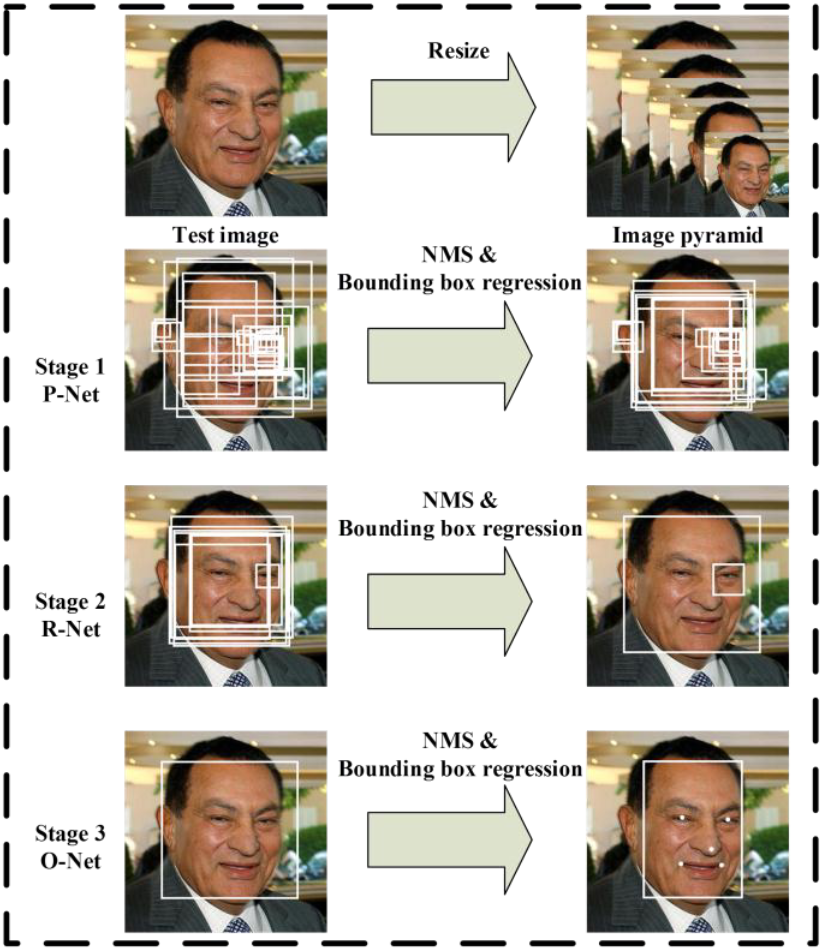
\includegraphics[width=\textwidth]{mtcnn.png}
      \label{fig:mtcnn}
    \end{minipage}
    \hspace{0.5cm}
    \begin{minipage}[c]{0.52\textwidth}
      \centering
      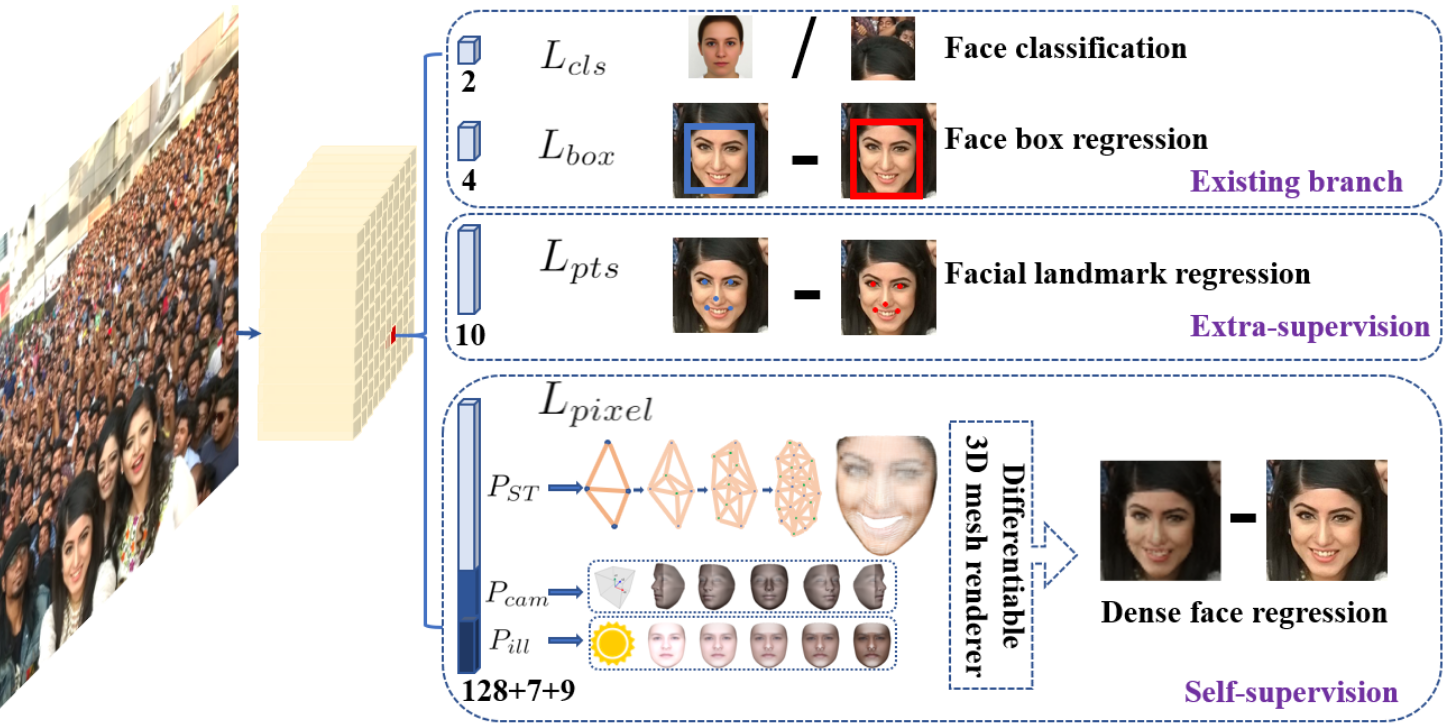
\includegraphics[width=\textwidth]{retinaface.png}
      \label{fig:retinaface}
    \end{minipage} 
    \begin{minipage}{0.4\textwidth}
        \vspace{-0.5cm}
        \centering
        \footnotesize a)
    \end{minipage}
    \hfill
    \begin{minipage}{0.4\textwidth}
        \vspace{-0.5cm}
        \centering
        \footnotesize b)
    \end{minipage}
    \vspace{-0.4cm}
    \caption{Comparison between \textbf{a)} MTCNN: multi-stage, CPU real-time and multi-task learning, and \textbf{b)} RetinaFace: single-stage, anchor-based, CPU real-time and multi-task learning. MTCNN \autocite{zhangJointFaceDetection2016a} proposes a series of bounding boxes then, through a series of refinement stages, the best solution and landmarks are found. RetinaFace \autocite{dengRetinaFaceSinglestageDense2019} accomplishes, in a single-stage, face classification and bounding box regression by evaluating anchors, landmark localization and dense 3D projection for facial correspondence.}
    \label{fig:mtcnn vs retinaface}
\end{figure}
  

\noindent\textbf{$\rightarrow$ Multi-stage} methods \autocite{dengRetinaFaceSinglestageDense2019} include all the coarse-to-fine facial detectors that work in similar manner to the following two phases. First, bounding box proposals are generated by sliding a window through the input. Then, over one or several subsequent stages, false positives are rejected and the approved bounding boxes are refined. To complement, one widely applied object detection protocol that inspired face detection methods and perfectly describes the steps mentioned above is Faster R-CNN \autocite{renFasterRCNNRealTime2016}. However, these methods can be slower and have a more complex way of training \autocite{xuCenterFaceJointFace2019}.

\vspace{0.7\baselineskip}
\noindent\textbf{$\rightarrow$ Single-stage} approaches \autocite{dengRetinaFaceSinglestageDense2019} are the ones that perform classification and bounding box regression without the necessity of a proposal stage, producing highly dense face locations and scales. This structure takes inspiration, once again, from general object detectors, for example, the Single Shot MultiBox detector, commonly referred to as SSD \autocite{liuSSDSingleShot2016}. Finally, the methods included in this class are more efficient, but can incur in compromised accuracy, when compared to multi-stage.

\vspace{0.7\baselineskip}
\noindent\textbf{$\rightarrow$ Anchor-based} techniques \autocite{liuHAMBoxDelvingOnline2019, dengRetinaFaceSinglestageDense2019, zhangFaceDetectionUsing2018} detect faces by predefining anchors with different settings (scales, strides, number, etc.) on the feature maps, then performing classification and bounding box regression on them until an acceptable output is found. As proven by Liu and Tang \textit{et al.} \autocite{liuHAMBoxDelvingOnline2019}, the choice of anchors highly influences the results of prediction. Hence, it is necessary to fine-tune them on a situation-by-situation basis, otherwise, there is a limitation in generalization. Furthermore, higher densities of anchors directly generate an increase in computational overhead.

\vspace{0.7\baselineskip}
\noindent\textbf{$\rightarrow$ Anchor-free} procedures, obviously, do not need predefined anchors in order to find faces. Alternatively, these methods address the face detection by using different techniques. For example, DenseBox \autocite{huangDenseBoxUnifyingLandmark2015} which attempts to predict faces by processing each pixel as a bounding box, or CenterFace \autocite{xuCenterFaceJointFace2019} that treats face detection as a key-point estimation problem by predicting the center of the face and bounding boxes. Even so, relating to the accuracy of anchor-free approaches, there's still room for improvement for false positives and stability in the training stage \autocite{duElementsEndtoendDeep2022}.

\vspace{0.7\baselineskip}
\phantomsection\label{mt learning}
\noindent\textbf{$\rightarrow$ Multi-task learning} are all the methodologies that conjointly performs other tasks, namely facial landmark\footnote{A facial landmark is a key-point in a face that contributes with important geometric information, namely the eyes, nose, mouth, etc. \autocite{fengWingLossRobust2018}} localization, during face classification and bounding box regression \autocite{duElementsEndtoendDeep2022}. CenterFace \autocite{xuCenterFaceJointFace2019} is one example, and so it is the widely implemented MTCNN \autocite{zhangJointFaceDetection2016a}, which correlated bounding boxes and face landmarks. RetinaFace \autocite{dengRetinaFaceSinglestageDense2019} is another state-of-the-art approach, it mutually detects faces, respective landmarks and performs dense 3D face regression.

\vspace{0.7\baselineskip}
\noindent\textbf{$\rightarrow$ CPU real-time} methods, as the name suggests, include the detectors that can run on a single CPU core, in real-time, for VGA-resolution input images. A face detector can achieve great results in terms of accuracy, but for real world applications, its use can be too computational heavy, therefore, can't be deployed in real time (specially in devices that do not have a GPU) \autocite{duElementsEndtoendDeep2022}. MTCNN \autocite{zhangJointFaceDetection2016a}, Faceboxes \autocite{zhangFaceBoxesCPURealtime2018}, CenterFace \autocite{xuCenterFaceJointFace2019} or RetinaFace \autocite{dengRetinaFaceSinglestageDense2019} are examples of this category.

\vspace{0.7\baselineskip}
\noindent\textbf{$\rightarrow$ Problem-oriented} is a category that includes the detectors that are projected to resolve a wide range of specific problems, for example, faces that are tiny, partially occluded, blurred or scale-invariant face detection \autocite{duElementsEndtoendDeep2022}. PyramidBox \autocite{tangPyramidBoxContextassistedSingle2018} is an example that solves the partial occluded and blurry faces, and HR \autocite{huFindingTinyFaces2017} tackles the tiny faces challenge.

\vspace{0.7\baselineskip}
Although this distribution can create some overlap among the categories, it is superior due to the simplicity of inferring what defines each category and being a more fine-grained way of classifying techniques when compared to others, namely the dual categorical division by \autocite{ranjanDeepLearningUnderstanding2018} that groups the methods in region\footnote{Region-based approaches creates thousands of generic object-proposals for every image, and subsequently, a DCNN classifies if a face is present in any of them.} or sliding-window\footnote{Sliding-window approaches centers on using a DCNN to compute a face detection score and bounding box at every location in a feature map.} based. 

\subsection{Face Alignment}
\par Face Alignment, or facial landmark detection \autocite{changFacePoseNetMakingCase2017}, is the second stage of the face recognition pipeline, and has the objective of calibrating the detected face to a canonical layout, through landmark-based or landmark-free approaches, in order to leverage the core final stage of face representation \autocite{duElementsEndtoendDeep2022}. 
\par Despite the fact that traditional face alignment methods are very accurate, that only occurs in constrained circumstances. Therefore, once again, to address that issue, deep learning-based methods are the solution to perform an accurate facial landmark localization that realistically scales to real world scenarios \autocite{fengWingLossRobust2018}. 
\par Furthermore, face alignment, can be accomplished through two categories of methods: landmark-based and landmark-free.

\vspace{0.7\baselineskip}
\noindent\textbf{$\rightarrow$ Landmark-based alignment} is a category of methods that exploits the facial landmarks with the aim of, through spatial transformations, calibrating the face to an established layout \autocite{duElementsEndtoendDeep2022}. This can be accomplished through: coordinate regression, heatmap regression or 3D Model Fitting. \textbf{Coordinate regression-based} methodologies \autocite{fengWingLossRobust2018,liuTwoStreamTransformerNetworks2018,zhangJointFaceDetection2016a} consider the landmark localization as a numerical objective, i.e. a regression, thus an image is fed to a DCNN and it will output a vector of landmark coordinates. \textbf{Heatmap Regression} \autocite{dengJointMultiviewFace2017,wuLookBoundaryBoundaryAware2018,chenFaceAlignmentKernel2019} is different from coordinate regression because, although it is a numerical objective task, the output is not a coordinate vector, but a map of likelihood of landmarks' locations. Finally, \textbf{3D Model Fitting} \autocite{bhagavatulaFasterRealtimeFacial2017,changFacePoseNetMakingCase2017,xiaoRecurrent3D2DDual2017}is the category that integrates methods that consider the relation between 2D facial landmarks and the 3D shape of a generic face. The particularity of them is the reconstruction of the 3D face from a 2D face image that is then projected over a plane in order to obtain the landmarks. 

\vspace{0.7\baselineskip}
\noindent\textbf{$\rightarrow$ Landmark-free alignment}, on the other hand, integrates the approaches that do not rely on landmarks as a reference to align the face, in contrast, these type of methods incorporate the alignment into a DCNN that gives, as a result, an aligned face \autocite{duElementsEndtoendDeep2022}. An example of an end-to-end method that does not depend on facial landmarks is RDCFace \autocite{zhaoRDCFaceRadialDistortion2020}, and it rectifies distortions, applies alignment transformations and executes face representation. Hayat et al. \autocite{hayatJointRegistrationRepresentation2017} proposes a method that deals with extreme head poses. The process to register faces in an image with high pose variance can be quite challenging and often demands complex pre-processing, namely landmark localization, therefore, to address that, a DCNN is employed that does not rely on landmark localization and concomitantly register and represent faces.

%A facial landmark is nothing more than an important geometric point of reference that facilitates the alignment by acting as a reference

\vspace{0.7\baselineskip}
\par As can be seen from the previous section, this step in the face recognition process can be accomplished, very sporadically, through standalone methods that process the detected face from the previous stage, but generally joint detection and alignment methods (and sometimes even face representation), previously referenced in the \hyperref[mt learning]{multi-task learning} definition, are the optimal choice \autocite{changFacePoseNetMakingCase2017}.

\subsection{Face Representation}
\par Finally, Face Representation is the last stage of the Face Recognition process. It is responsible for processing the aligned face from the previous stage and mapping the produced feature representation to a feature space, in which features from the same person are closer together and those that are different stand further apart from each other \autocite{duElementsEndtoendDeep2022}.
\par According to the literature \autocite{duElementsEndtoendDeep2022,liHandbookFaceRecognition2011,ranjanDeepLearningUnderstanding2018,schroffFaceNetUnifiedEmbedding2015,wangDeepFaceRecognition2021}, there's a consensus about how Face Recognition can be performed in two settings of operation: face verification and face identification. This distinction is only made possible due to the approaches available in the Face Representation stage that can leverage one, the other or both. 

\vspace{0.7\baselineskip}
\noindent\textbf{$\rightarrow$ Face verification}, also referred to as \textbf{face authentication}, is a one-to-one match, and it's the action of verifying if the query face matches the identity that's being claimed. \red{These principles are used in biometric systems such as self-service immigration clearance using E-passport.} \autocite{liHandbookFaceRecognition2011}

\vspace{0.7\baselineskip}
\noindent\textbf{$\rightarrow$ Face identification}, also called \textbf{face recognition}, is a one-to-many correlation process that compares a query face to a database of faces and associates it to the corresponding match (or matches). \red{A typical use case is to identify someone in a watchlist or surveillance videos.} \autocite{liHandbookFaceRecognition2011}

\vspace{0.7\baselineskip}
\par The overall pipeline comes to a conclusion in this module, however, in reality, it goes further than that. As can be seen in \reffig{fig:fr pipeline}, due to its importance for the face recognition problem, it's highlighted the inherent pipeline of the Face Representation stage, henceforth, it shall be discussed in depth in the next section.

\newpage
\section{Face Representation Pipeline}
\begin{figure}[!h]
    \centering
    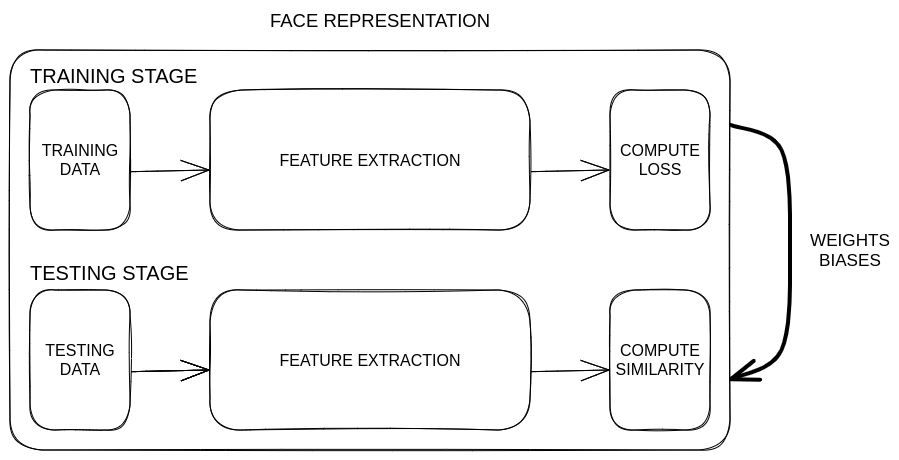
\includegraphics[scale=0.4]{frep_pipeline.png}
    \caption[Pipeline]{Face Representation pipeline, guided by the approach in \autocite{wangDeepFaceRecognition2021}.}
    \label{fig:frep pipeline}
\end{figure}

\par As show in \reffig{fig:frep pipeline}, Face Representation is a two-step module composed of a training and testing stage. So as to be capable of performing face recognition, in either a verification or identification manner, a face representation system needs to learn robust, invariant and discriminative features that can distinguish identities \autocite{ranjanDeepLearningUnderstanding2018}. 
\par To meet these requirements, the feature extractor must first be trained properly by taking data from previous stages and outputting a feature representation that's compared to the desired value using a loss function\footnote{Also referred to as a cost or objective function. \autocite{lecunDeepLearning2015}} \autocite{lecunDeepLearning2015, wangDeepFaceRecognition2021}. After that, everything is ready for the testing stage, where the face recognition \textit{per se} occurs by calculating a similarity score for the feature representation produced by the trained feature extractor, and dictating if the identity belongs to the same person (face verification) or if it matches any identity (face identification) \autocite{ranjanDeepLearningUnderstanding2018}.



\subsection{Datasets: Training and Testing Data}
\par As been discussed throughout this dissertation, Deep Learning techniques can solve the problem of handling unconstrained scenarios, where there are variations in pose, illumination, occlusion, and so forth. To support this, in the past few years, datasets have been developed with this in mind so to be able to provide a large and diverse set of both training data, allowing for adequate regularization to unseen circumstances, and testing data that benchmarks the face recognition system in, as similar as possible, unconstrained real world scenarios \autocite{duElementsEndtoendDeep2022}. 

\subsubsection{\large Training Data}
\par When developing a deep face recognition system it's essential to keep in mind its necessity to adapt, and that's where the dataset used for training comes at play. Large training datasets are essential for face recognition \autocite{parkhiDeepFaceRecognition2015}, but large-scale is not enough. There must be a balance between the depth (number of unique identities) and the breadth/width (number of images per identity) \autocite{bansalDonTsCNNbased2017, caoVGGFace2DatasetRecognising2018}, and it will lead to different effects. 
\par On one hand, a training dataset that is deep will help the face recognition system to produce more discriminative feature representations, since it will have a great number of identities to learn from. On the other hand, a wider set will have more images per identity, therefore, variations in pose, expressions, illuminations, occlusions, background clutter, image quality, accessories, and so forth \autocite{baeDigiFace1MMillionDigital2023} can be introduced and ultimately lead to feature representations more robust to them.

\vspace{\baselineskip}
In the following pages, a mix of training datasets, of overall relevance and more geared towards the purpose of this dissertation, will be reviewed.

% \par Earlier works \autocite{schroffFaceNetUnifiedEmbedding2015,sunDeepLearningFace2014,taigmanDeepFaceClosingGap2014} resourced private face datasets, but as time passed, more public datasets were released. 

\vspace{0.7\baselineskip}
\noindent\textbf{$\rightarrow$ CASIA-WebFace} \autocite{yiLearningFaceRepresentation2014}, composed of 494,414 face images and 10,575 identities, was proposed as a novel dataset to overcome the problem of data dependence in face recognition and improve comparability across different methods. By training on the same dataset, methods can be better evaluated and compared.

\vspace{0.7\baselineskip}
\noindent\textbf{$\rightarrow$ VGGFace} \autocite{parkhiDeepFaceRecognition2015} was published alongside a homonymous face recognition method and, once again, with the objective of combating the lack of available large scale public datasets. It contains 2,6 million images and 2,622 different identities and a curated version, where incorrect image labels were hand-removed by humans, has 800,000 images for the same amount of identities.

% Both datasets were released for training only purposes \autocite{caoVGGFace2DatasetRecognising2018}.

% \vspace{0.7\baselineskip}
% \noindent\textbf{$\rightarrow$ CelebA} 2015

% \vspace{0.7\baselineskip}
% \noindent\textbf{$\rightarrow$ UMDFaces} 2015

\vspace{0.7\baselineskip}
\noindent\textbf{$\rightarrow$ MS-Celeb-1M}'s \autocite{guoMSCeleb1MDatasetBenchmark2016} first intention was to provide a novel benchmark to identify celebrities that solves name ambiguities by linking a face with an entity key in a knowledge base. Second, it aimed at solving the gap in available large-scale datasets by providing a training set with, approximately, 10 million images and 100 thousand identities. Unfortunately, it is a dataset known for the presence of noisy labels. 

% That is mainly due to the size of the dataset, the automatic method of collecting and annotating the images, and also the fact that the noise is not removed on purpose (under the assumption that training with noisy data might be beneficial). 

\vspace{0.7\baselineskip}
\noindent\textbf{$\rightarrow$ MegaFace} \autocite{nechLevelPlayingField2017} introduced a benchmark for million-scale face recognition and provided a public large-scale training dataset that integrated 4,753,320 faces over 672,057 identities. The main difference compared to the previously mentioned datasets is that MegaFace does not use celebrities as subjects, in contrast it leverages the photographs released by Flickr under the Creative Commons license. 

\vspace{0.7\baselineskip}
\noindent\textbf{$\rightarrow$ VGGFace2} \autocite{caoVGGFace2DatasetRecognising2018} is another large-scale dataset, and its main goals are: 1) covering numerous identities, 2) reduce labeling noise through automatic and manual filtering and, finally, 3) represent more realistic unconstrained scenarios due to a novel dataset generation pipeline that gathers images with a broad range of poses, age, illumination and ethnicity. All in all, this resulted in a dataset comprised of 3,31 million faces of 9131 subjects.

\vspace{0.7\baselineskip}
\noindent\textbf{$\rightarrow$ UMDFaces-Videos} \autocite{bansalDonTsCNNbased2017} is a video-based dataset composed of 22,075 videos of 3,107 subjects with 3,735,476 human annotated frames with great variation in image quality, pose, expressions and lightning. It was proposed during a study how the performance of a face verification models is impacted by the effects of: 1) the type of media used for training (only videos or still images vs a mixture of both), 2) the width and depth of a dataset, 3) the label's noise and 4) the alignment of the faces.


% training on a mixture of still images and videos boosts performance. There's a bias toward high quality images in still datasets due to the way of capturing the data (high quality cameras). Models trained only on still images perform poorly on frames extracted from videos, they're very challenging due to pose, expression and illumination variations. Models trained only on videos perform poorly on datasets composed of only still images.

% The introduction of noisy labels does not increase face verification performance, clean data always performs better. Although, the difference between a clean dataset and one with a low percentage of noise (less than 5\%) is very low.

\vspace{0.7\baselineskip}
\noindent\textbf{$\rightarrow$ Celeb-500k} \autocite{caoCeleb500KLargeTraining2018} is another large-scale proposed with two issues in mind: the disparity in the scale of public datasets when compared with private ones, and determining the impact in performance from intra- and inter-class variations. That being so, Celeb-500k, consisting of 50 million images from 500 thousand persons, and Celeb-500k-2R, a cleaned version of the previous, comprised of 25 million aligned faces of 245 thousand identities, are released.

\vspace{0.7\baselineskip}
\noindent\textbf{$\rightarrow$ IMDb-Face} \autocite{wangDevilFaceRecognition2018} proposes a new dataset with based on a manually cleaned revision of MS-Celeb-1M and MegaFace. The growing demand for large-scale datasets introduced a new variable to take into consideration: the time available to annotate the data. Datasets that are well-annotated and have an enormous amount of data are notably expensive and time-consuming to develop. Therefore, automatic measures to clean the data were used, so it's expected for a certain degree of noise to be introduced in a dataset. After selecting a subset from both the originals datasets, 2 million images were manually cleaned and resulted in 1,7 million images of 59 thousand celebrities.

\vspace{0.7\baselineskip}
\noindent\textbf{$\rightarrow$ MS1MV2} \autocite{dengArcFaceAdditiveAngular} is another well know dataset. It was proposed in the ArcFace face recognition method paper and consists of a semi-automatic refinement of the previously mentioned MS-Celeb-1M, resulting in 5,8 million images of 85 thousand identities.

\vspace{0.7\baselineskip}
\noindent\textbf{$\rightarrow$ MS1M-RetinaFace} \autocite{dengLightweightFaceRecognition2019} is a semi-automatically refined version of MS-Celeb-1M using the ArcFace method with ethnicity-specific annotators. This resulted in 5,1M faces of 93k identities.

\vspace{0.7\baselineskip}
\noindent\textbf{$\rightarrow$ RMFRD} \autocite{wangMaskedFaceRecognition2020} is presented in the context of the need of using a mask, mandated by the COVID-19 pandemic, and that greatly reduces the effectiveness of conventional face recognition methods. Therefore, there was a need to improve their performance and for that a dataset that provides masked faces is needed. RMFRD pioneered this need by publishing a dataset consisting of 5 thousand masked and 90 thousand unmasked faces from 525 celebrities.

\vspace{0.7\baselineskip}
\noindent\textbf{$\rightarrow$ Glint360K} \autocite{anPartialFCTraining2021} is a training set presented in the Partial FC method paper. It was generated by merging and cleaning the aforementioned Celeb-500K and MS1MV2 datasets, which resulted in 17 million images of 360 thousand individuals.

\vspace{0.7\baselineskip}
\noindent\textbf{$\rightarrow$ WebFace260M} \autocite{zhuWebFace260MBenchmarkUnveiling2021} takes a giant leap in closing the gap between public available datasets and private ones. Partnered with a time-constrained face recognition protocol, the original paper presented an enormous 260 million faces and 4 million identities noisy dataset, an automatically cleaned, high quality training set with 42 million faces over 2 million identities (WebFace42M), and a smaller scale training dataset derived from the WebFace42M that has 10\% of its data (WebFace4M).
 % Traditional test datasets that focus on accuracy have been almost saturated
 % Interesting time-constrained face recognition protocol

\vspace{0.7\baselineskip}
\noindent\textbf{$\rightarrow$ DigiFace-1M} \autocite{baeDigiFace1MMillionDigital2023} is a novel approach that revolutionizes the way of training face recognition models. It is a fully synthetic dataset that proposes mitigating three very relevant problems present in the majority of the conventional datasets: 1) ethical issues, 2) label noise and 3) data bias. The dataset is divided in two parts: part one contains 720 thousand images from 10 thousand identities and part two has 500 thousand images with 100 thousand identities, for a total of 1,22 million images and 110 thousand unique identities.

% Privacy violations, lack of informed consent and exploitation of distribution licenses or vague terms (such as "celebrities") to gather data are some of the criticisms that raised enough concerns that lead to revoking the distribution of several datasets. 

\begin{table}[!ht]
    \centering
    \resizebox{\textwidth}{!}{%
    \begin{tabular}{|l|c|c|c|c|c|c|c|}
    \hline
    \multicolumn{1}{|c|}{\textbf{Dataset}} & \textbf{Year} & \textbf{Availability} & \textbf{Images/videos} & \textbf{Depth} & \textbf{Avg. Breadth} & \textbf{Distribution} & \textbf{Description} \\ \hline
    CASIA-WebFace \autocite{yiLearningFaceRepresentation2014}                         & 2014          & Discontinued          & 494,414/-              & 10,575         & 46.7                  & Public                & First public face recognition dataset.                 \\ \hline
    \textit{Facebook} \autocite{taigmanWebscaleTrainingFace2015}                               & 2015          & -                     & 500M/-                 & 10M            & 50                    & Private               & \textit{Facebook}'s private dataset used to test different properties in face identification.                 \\ \hline
    \textit{Google} \autocite{schroffFaceNetUnifiedEmbedding2015}                                 & 2015          & -                     & 200M/-                 & 8M             & 25                    & Private               & Private dataset used to train the FaceNet method.                 \\ \hline
    VGGFace \autocite{parkhiDeepFaceRecognition2015}                                & 2015          & Discontinued          & 2,6M/-                 & 2,622          & 991.6                 & Public                & High width public dataset released alongside VGGFace method.                 \\ \hline
    MS-Celeb-1M \autocite{guoMSCeleb1MDatasetBenchmark2016}                           & 2016          & Discontinued          & 10M/-                  & 100k           & 100                   & Public                & Large-scale celebrities dataset.                 \\ \hline
    MegaFace \autocite{nechLevelPlayingField2017}                               & 2016          & temp                  & 4,753,320/-            & 672,057        & 7.1                   & Public                & Non-celebrity dataset.                 \\ \hline
    VGGFace2 \autocite{caoVGGFace2DatasetRecognising2018}                               & 2017          & temp                  & 3,31M/-                & 9131           & 362.5                 & Public                & High characteristics variation dataset.                 \\ \hline
    UMDFaces-Videos \autocite{bansalDonTsCNNbased2017}                        & 2017          & temp                  & -/22,075               & 3,107          & 7.1                   & Public                & Video-based dataset with great variations.                 \\ \hline
    Celeb-500k \autocite{caoCeleb500KLargeTraining2018}                             & 2018          & temp                  & 50M/-                  & 500k           & 100                   & Public                & Noisy celebrities dataset.                 \\ \hline
    Celeb-500k-2R \autocite{caoCeleb500KLargeTraining2018}                          & 2018          & temp                  & 25M/-                  & 245k           & 102                   & Public                & Cleaned version.                 \\ \hline
    IMDb-Face \autocite{wangDevilFaceRecognition2018}                              & 2018          & temp                  & 1,7M/-                 & 59k            & 28.8                  & Public                & Manually cleaned revision of MS-Celeb-1M and MegaFace.                 \\ \hline
    MS1MV2 \autocite{dengArcFaceAdditiveAngular}                                 & 2019          & temp                  & 5,8M/-                 & 85k            & 68.2                  & Public                & Semi-automatic cleaned version of MS-Celeb-1M.                 \\ \hline
    MS1M-RetinaFace \autocite{dengLightweightFaceRecognition2019}                                 & 2019          & temp                  & 5,1M/-                 & 93k            & 54.8                  & Public                & Semi-automatic cleaned version of MS-Celeb-1M.                 \\ \hline
    RMFRD \autocite{wangMaskedFaceRecognition2020}                                 & 2020          & temp                  & 95k/-                  & 525            & 180.9                 & Public                & Dataset of masked and unmasked celebrities.                 \\ \hline
    Glint360k \autocite{anPartialFCTraining2021}                              & 2021          & temp                  & 17M/-                  & 360k           & 47.2                  & Public                & Cleaned version of the Celeb-500k AND MS1MV2 datasets.                \\ \hline
    WebFace260M \autocite{zhuWebFace260MBenchmarkUnveiling2021}                            & 2021          & temp                  & 260M/-                 & 4M             & 65                    & Public                & Largest publicly available dataset of celebrities faces (noisy).                 \\ \hline
    WebFace42M \autocite{zhuWebFace260MBenchmarkUnveiling2021}                             & 2021          & temp                  & 42M/-                  & 2M             & 21                    & Public                & Cleaned and smaller version.                 \\ \hline
    WebFace4M \autocite{zhuWebFace260MBenchmarkUnveiling2021}                              & 2021          & temp                  & 4,2M/-                 & 200k           & 21                    & Public                & Smaller version.                 \\ \hline
    DigiFace-1M \autocite{baeDigiFace1MMillionDigital2023}                            & 2022          & Available                  & 1,22M/-                & 110k           & 11.1                  & Public                & Large-scale, fully synthetic dataset.                 \\ \hline
    \end{tabular}%
    }
    \caption{Oof}
    \label{tab:training data}
\end{table}
\newpage
\subsubsection{\large Testing Data}

\par After the training is completed the performance of the system needs to be evaluated on different challenges to properly access if it scales (or generalizes or applies or performs in) to real-world scenarios. A test dataset can be chosen for specific hurdles, for instance, cross-pose, cross-age, racial variations, quality assessment, and so forth \autocite{duElementsEndtoendDeep2022}.


\vspace{0.7\baselineskip}
\noindent\textbf{$\rightarrow$ LFW} \autocite{huangLabeledFacesWild} is the most well-known face verification dataset. It was first released in 2007 as a way of evaluating the performance of face recognition methods, in a verification or pair matching manner, under unconstrained scenarios. LFW divides the dataset in 2 views. View 1 is designed for development, and in the training set contains 1100 pairs of mismatched images and 1100 pairs of matched ones, while the test set has 500 pairs of matched and 500 pairs of unmatched faces. View 2 is intended for performance reporting and splits the data over 10 separate sets, to facilitate 10-fold cross validation, where each one has 300 positive pairs (same identity) and 300 negative pairs (different person), resulting in 6000 pairs. Overall, the dataset has 13,233 face images and 5749 identities (only 1680 persons have two or more images).

\vspace{0.7\baselineskip}
\noindent\textbf{$\rightarrow$ YTF} \autocite{wolfFaceRecognitionUnconstrained2011} is a video-based benchmark that leverages the greater amount of information provided by a video in comparison to still images. By collecting videos from \textit{Youtube} there isn't an opportunity to control the conditions, hence the footage will support a wider range of characteristic's variation, namely lighting conditions, difficult poses, motion blur, compression artifacts, etc. This resulted in 3425 videos from 1595 identities and a benchmark protocol inspired in the LFW. To evaluate performance, a pair-matching test is designed. From the database, 5000 video pairs are collected, where half are matches and the other half are not, to be divided to allow 10-fold cross validation.

\vspace{0.7\baselineskip}
\noindent\textbf{$\rightarrow$ IJB-A} \autocite{klarePushingFrontiersUnconstrained2015} aims at straying further from the saturation in recognition benchmarks by proposing more challenging benchmarks (specifically by including wider geographic distribution and full pose variation) for both verification and identification. It consists of a mix of 5712 images and 2085 videos from 500 individuals, with manual bounding boxes, facial landmarks and, most importantly, labels. IJB-A supports two protocols: search (face identification) and compare (face verification). For both the protocols, the specifications are the same, i.e., ten random training and testing splits are generated using all 500 identities then used to perform sample bootstrapping (instead of cross validation) in order to enhance the number of testing subjects. For each split, 333 subjects are randomly distributed in the training set and the remainder 167 are placed in the testing set.

\vspace{0.7\baselineskip}
\noindent\textbf{$\rightarrow$ CFP} \autocite{senguptaFrontalProfileFace2016} studies the effect of extreme pose variations, such as a profile view of a face, in face verification. During collection gender and profession balance, as well as racial diversity, were considered. A number of frontal and profile view images was also set as 10 and 4, respectively. Therefore, after cleaning the initial data, it resulted in 7000 images from 500 subjects. The experimental protocol divided the 500 identities over 10 splits (facilitating 10-fold cross validation) and randomly generated 7 matched pairs and 7 unmatched pairs per identity, resulting in a total of 7000 pairs of faces.

\vspace{0.7\baselineskip}
\noindent\textbf{$\rightarrow$ MegaFace2} \autocite{nechLevelPlayingField2017} has already been mentioned in the Training Data section, with exception to detailing the benchmarking protocol. The MegaFace2 is used to train the model that will be tested in 3 datasets: a one million Flickr distraction set, FaceScrub \autocite{ngDatadrivenApproachCleaning2014} and FG-Net. The first dataset is intended to supply the model with identities that are not to be found (hence being called a distraction set), while the last two contain the known identities to be tested.

\vspace{0.7\baselineskip}
\noindent\textbf{$\rightarrow$ CPLFW} \autocite{zhengCrossPoseLFWDatabase} is another dataset that tackles the overly optimistic accuracy saturation in classic benchmarks, such as the previously mentioned LFW. To this end, evaluating performance for cross-pose faces of LFW subjects is the matter of study. It contains the same number of 13,233 images of 5749 identities like LFW and the benchmark protocol performance is the LFW \textit{View 2} with some differences: 1) negative pairs are from people of the same race and gender, 2) class imbalance and limited positive pair's diversity is resolved by assuring that each identity has at least 2 images.

\vspace{0.7\baselineskip}
\noindent\textbf{$\rightarrow$ CALFW} \autocite{zhengCrossAgeLFWDatabase2017} has the same principles as CPLFW but applied to the age of the subjects (including the negative pairs selection and the class imbalance).

\vspace{0.7\baselineskip}
\noindent\textbf{$\rightarrow$ Age-DB} \autocite{moschoglouAgeDBFirstManually2017}, similarly to CALFW, is a dataset that considers the subject's age. It distances from other databases by solving the noisy labelling, induced by automatic or semi-automatic methods, by doing so manually. Age-DB has 16,488 images and 568 subjects used in 4 evaluation protocols, similar to LFW's \textit{View 2}, where the main difference between them is the age difference between pairs (5, 10, 20 and 30 years).

\vspace{0.7\baselineskip}
\noindent\textbf{$\rightarrow$ IJB-B} \autocite{whitelamIARPAJanusBenchmarkB2017} builds upon IJB-A and proposes solving flaws that were verified in the previous dataset. First, the improved IJB-B dataset is larger, consisting of 21,798 images and 7,011 videos from 1,845 subjects, with a more uniform racial distribution. Second, the protocols are upgraded due a greater number of possible comparisons between images and possible identities.

\vspace{0.7\baselineskip}
\noindent\textbf{$\rightarrow$ TinyFace}

\vspace{0.7\baselineskip}
\noindent\textbf{$\rightarrow$ IJB-C} 

\vspace{0.7\baselineskip}
\noindent\textbf{$\rightarrow$ IJB-S}

\vspace{0.7\baselineskip}
\noindent\textbf{$\rightarrow$ RFW}

\vspace{0.7\baselineskip}
\noindent\textbf{$\rightarrow$ QMUL-SurvFace} \autocite{chengSurveillanceFaceRecognition2018} is a dataset introduced as a benchmark in the \textit{Surveillance Face recognition Challenge} for face recognition in a surveillance context. By data-mining 17 public person re-identification datasets, it achieves 463,507 facial images of 15,573 identities collected in uncooperative surveillance scenarios. Consequently, it presents a high variance in resolution, motion blur, pose, occlusion, illumination and background clutter.

\vspace{0.7\baselineskip}
\noindent\textbf{$\rightarrow$ CAFR} \autocite{zhaoAgeInvariantFaceRecognition2022}

\vspace{0.7\baselineskip}
\noindent\textbf{$\rightarrow$ MDMFR} \autocite{ullahNovelDeepMaskNetModel2022} is brought about in light of the COVID-19 impact, where wearing a mask became mandatory. Unfortunately, this rendered unusable the traditional face recognition methods because they were designed to recognize unveiled faces. Therefore, in conjunction with Deepmasknet, a framework that performs both masked detection and recognition, MDMFR was released

\vspace{0.7\baselineskip}
\noindent\textbf{$\rightarrow$ XQLFW}

\vspace{0.7\baselineskip}
\noindent\textbf{$\rightarrow$ FaVCI2D} 



\begin{table}[!ht]
    \centering
    \resizebox{\textwidth}{!}{%
    \begin{tabular}{|l|c|c|c|c|c|c|c|}
    \hline
    \multicolumn{1}{|c|}{\textbf{Dataset}} & \textbf{Year} & \textbf{Availability} & \textbf{Images/videos} & \textbf{Depth} & \textbf{Avg. Breadth} & \textbf{Distribution} & \textbf{Description} \\ \hline
    LFW \autocite{huangLabeledFacesWild}                                    & 2007          & Discontinued          & 494,414/-              & 10,575         & 46.7                  & Public                & temp                 \\ \hline
    YTF \autocite{wolfFaceRecognitionUnconstrained2011}                                    & 2011          & -                     & 500M/-                 & 10M            & 50                    & Private               & temp                 \\ \hline
    IJB-A \autocite{klarePushingFrontiersUnconstrained2015}                                  & 2015          & -                     & 200M/-                 & 8M             & 25                    & Private               & temp                 \\ \hline
    CFP \autocite{senguptaFrontalProfileFace2016}                                 & 2016          & Discontinued          & 2,6M/-                 & 2,622          & 991.6                 & Public                & temp                 \\ \hline
    MegaFace2* \autocite{nechLevelPlayingField2017}                              & 2016          & Discontinued          & 10M/-                  & 100k           & 100                   & Public                & temp                 \\ \hline
    CPLFW \autocite{zhengCrossPoseLFWDatabase}                                  & 2017          & temp                  & 4,753,320/-            & 672,057        & 7.1                   & Public                & temp                 \\ \hline
    CALFW \autocite{zhengCrossAgeLFWDatabase2017}                                  & 2017          & temp                  & 3,31M/-                & 9131           & 362.5                 & Public                & temp                 \\ \hline
    AgeDB \autocite{moschoglouAgeDBFirstManually2017}                                  & 2017          & temp                  & -/22,075               & 3,107          & 7.1                   & Public                & temp                 \\ \hline
    IJB-B \autocite{whitelamIARPAJanusBenchmarkB2017}                                 & 2017          & temp                  & 50M/-                  & 500k           & 100                   & Public                & temp                 \\ \hline
    TinyFace                               & 2018          & temp                  & 25M/-                  & 245k           & 102                   & Public                & temp                 \\ \hline
    IJB-C                                  & 2018          & temp                  & 1,7M/-                 & 59k            & 28.8                  & Public                & temp                 \\ \hline
    IJB-S                                  & 2018          & temp                  & 5,8M/-                 & 85k            & 68.2                  & Public                & temp                 \\ \hline
    RFW                                    & 2018          & temp                  & 95k/-                  & 525            & 180.9                 & Public                & temp                 \\ \hline
    QMUL-SurvFace                          & 2018          &                       &                        &                &                       &                       &                      \\ \hline
    CAFR                                   & 2020          &                       &                        &                &                       &                       &                      \\ \hline
    MDMFR                                  & 2021          &                       &                        &                &                       &                       &                      \\ \hline
    XQLFW                                  & 2021          & temp                  & 17M/-                  & 360k           & 47.2                  & Public                & temp                 \\ \hline
    FaVCI2D                                & 2022          & temp                  & 260M/-                 & 4M             & 65                    & Public                & temp                 \\ \hline
    \end{tabular}%
    }
    \caption{}
    \label{tab:test data}
\end{table}

\vspace{\baselineskip}
\par Although some of the previously referenced datasets do have a benchmarking component and are described as such, they can also be generally employed to train algorithms. When it is desired to finetune\footnote{Producing a new model for a specific task by freezing most of the model's layers and training only the last few \autocite{zhuangComprehensiveSurveyTransfer2020}. More details on this topic in the section \hyperref[transf learning]{Transfer Learning}.} a model for a specific challenge that, usually,  can be better achieved by employing a "benchmark" dataset that was purposefully developed to evaluate a model's performance on that exact challenge. 

\vspace{\baselineskip}
\centerline{
    \noindent
    \fbox{
        \begin{minipage}{0.95\textwidth}
            \centering
            \noindent A common denominator throughout the machine learning domain, and more specifically deep learning, is a general difficulty in separating concepts with a single line. This is a non-linear science in its nature.
        \end{minipage}
    }
}


\newpage
\subsection{Feature Extraction}

\begin{figure}[!h]
    \centering
    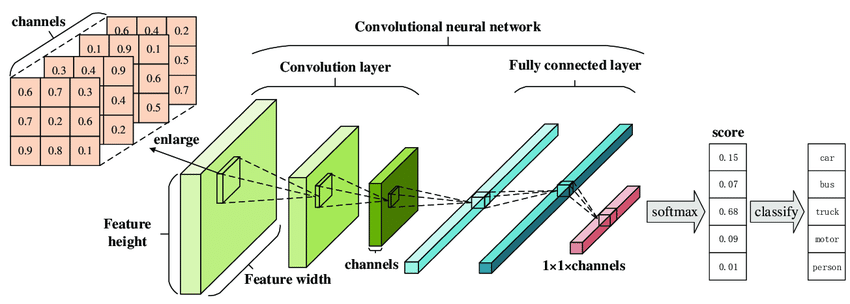
\includegraphics[width=0.85\textwidth]{Architecture-of-a-Convolutional-Neural-Network-CNN-The-traditional-CNN-structure-is.png}
    \caption{Architecture of a Convolutional Neural Network \autocite{kangDeepSimilarityMetric2019}.}
    \label{fig:cnn}
\end{figure}

There are several types of Neural Networks architectures, but Convolutional Neural Networks (CNNs or Convnets) are probably the most widely implemented model overall \autocite{yamashitaConvolutionalNeuralNetworks2018, liSurveyConvolutionalNeural2022} with successful applications in the domains of Computer Vision \autocite{krizhevskyImageNetClassificationDeep2012,taigmanDeepFaceClosingGap2014,tompsonEfficientObjectLocalization2015, zhangImprovedBreastCancer2021} or Natural Language Processing\autocite{abdel-hamidConvolutionalNeuralNetworks2014, wangGenCNNConvolutionalArchitecture2015, xiangConvolutionalNeuralNetworkbased2020}. In the CNN category itself there are different variants, but they all abide the fundamental structure of a feedforward hierarchical multi-layer network \reffig{fig:cnn}. Feedforward because the information only flows in a singular direction without cycling \autocite{zellSimulationNeuronalerNetze1994}, hierarchical because the higher complexity internal representations are learned from lower ones \autocite{lecunDeepLearning2015, zhuBCNNBranchConvolutional2017} and multi-layer because it is composed of a series of stages, blocks or layers: the raw data is fed to an input layer, forwarded to a sequence of intercalating convolutional and pooling layers, transmitted to a stage of one or more fully-connected layers \autocite{lecunDeepLearning2015, yamashitaConvolutionalNeuralNetworks2018, guRecentAdvancesConvolutional2018, alzubaidiReviewDeepLearning2021}. The convolutional layer is designed to extract feature representations by being composed of kernels (or filter banks \autocite{lecunDeepLearning2015}) that compute feature maps through element-wise product, to which is applied a nonlinear activation function \autocite{guRecentAdvancesConvolutional2018,yamashitaConvolutionalNeuralNetworks2018}. Next is the pooling layer, that's responsible for reducing the spatial size of the input data \autocite{guRecentAdvancesConvolutional2018} and joining identical features \autocite{lecunDeepLearning2015}. Finally, the fully connected layers, and their core function is to perform high logic and generate semantic information \autocite{guRecentAdvancesConvolutional2018}.


\par Using CNNs for Computer Vision tasks is not an arbitrary choice, but due to the fact that the network design can benefit from the intrinsic characteristics of the input data, consequently performing really well in image related applications \autocite{lecunDeepLearning2015,caoReviewNeuralNetworks2018}. In the first place, images have an array-like structure with numerous elements, namely, each pixel has an assigned value organized in a grid-like manner \autocite{yamashitaConvolutionalNeuralNetworks2018}. In the second place, there's an inherent correlation between local groups of values, which creates distinguishable motifs \autocite{lecunDeepLearning2015}. Finally, the local values of images are invariant to location, that is, a certain composition should have the same value independently of the spatial location in the picture \autocite{lecunDeepLearning2015}. Therefore, the following key, unique features potentiate the previously stated efficient performance \autocite{caoReviewNeuralNetworks2018}:
\begin{enumerate}
    \item Designed to process multidimensional arrays \autocite{lecunDeepLearning2015};
    \item Shared weights between the same features in different locations; %Invariance to shift, distortions and rotations
    \item Automatically identifies the relevant features without any human supervision, hence, small amounts of preprocessing \autocite{alzubaidiReviewDeepLearning2021,liSurveyConvolutionalNeural2022}; %Easier to train
    \item Local connections (or receptive fields/sparse connectivity) \autocite{alzubaidiReviewDeepLearning2021}; %Less complexity, easier to train; %Invariance to shift, distortions and rotations and less network complexity (easier to train)
    \item Pooling layers that reduces the spatial size of the input data. %Invariance to shift, distortions and rotations
\end{enumerate}
% Check this article for better description of key features \autocite{liSurveyConvolutionalNeural2022}

The ensemble of features 2, 4 and 5 enable an invariance of the network to small shifts, distortions and rotations \autocite{guRecentAdvancesConvolutional2018,lecunDeepLearning2015}, while 2, 3, 4 and 5 helps to reduce the complexity of the model, and as a result training it is easier\autocite{guRecentAdvancesConvolutional2018,liSurveyConvolutionalNeural2022}.

\phantomsection\label{transf learning}
\subsubsection{Transfer Learning}

\subsection{Loss}
\subsection{Similarity}

\end{document}